\section[\thesection \  Hardware]{Hardware}\label{sec:hardware}


\begin{frame}{Verwendete Hardware}
    \begin{columns}[T]

        \column{0.5\textwidth}
        \begin{itemize}
            \item Raspberry Pi 4
            \item Intels Neural Compute Stick 2
            \item Raspberry Pi Camera Modul mit IR Cut Funktion      
        \end{itemize}
        
        \column{0.5\textwidth}
        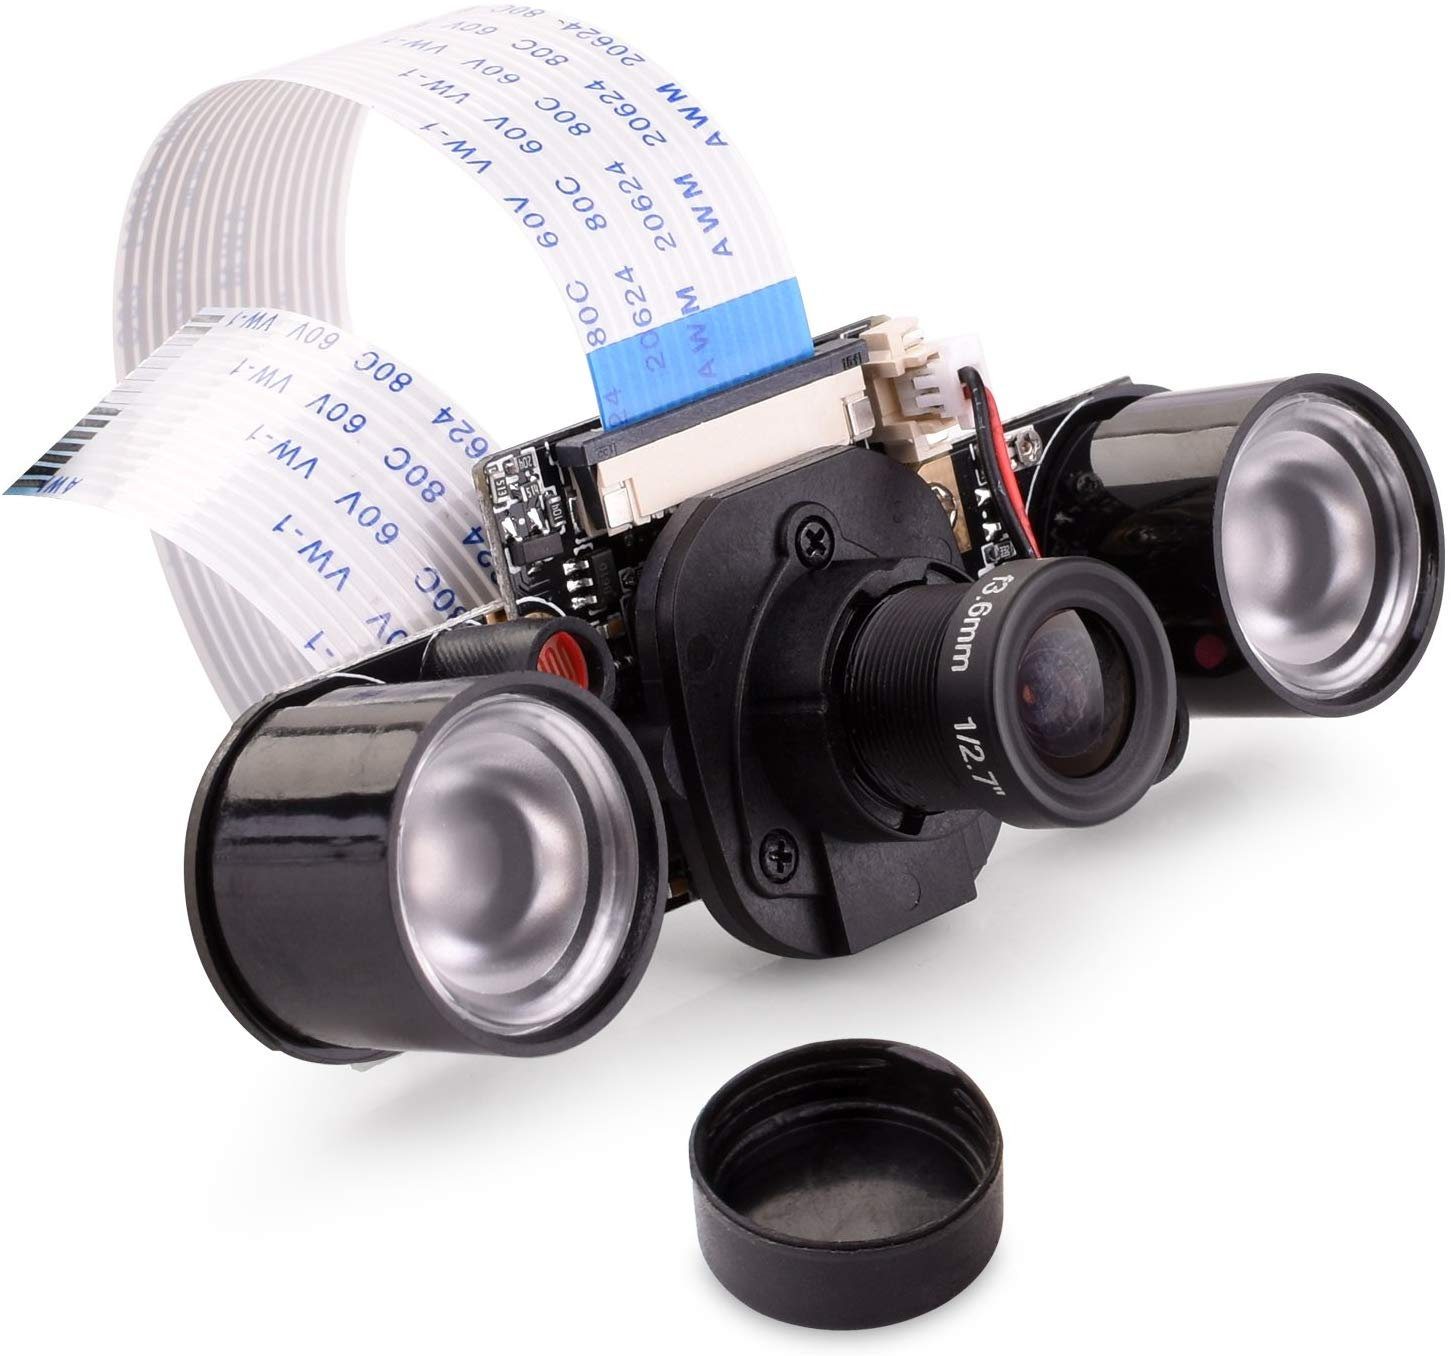
\includegraphics[width=0.6\textwidth]{Bilder/RPiCam.jpg}
        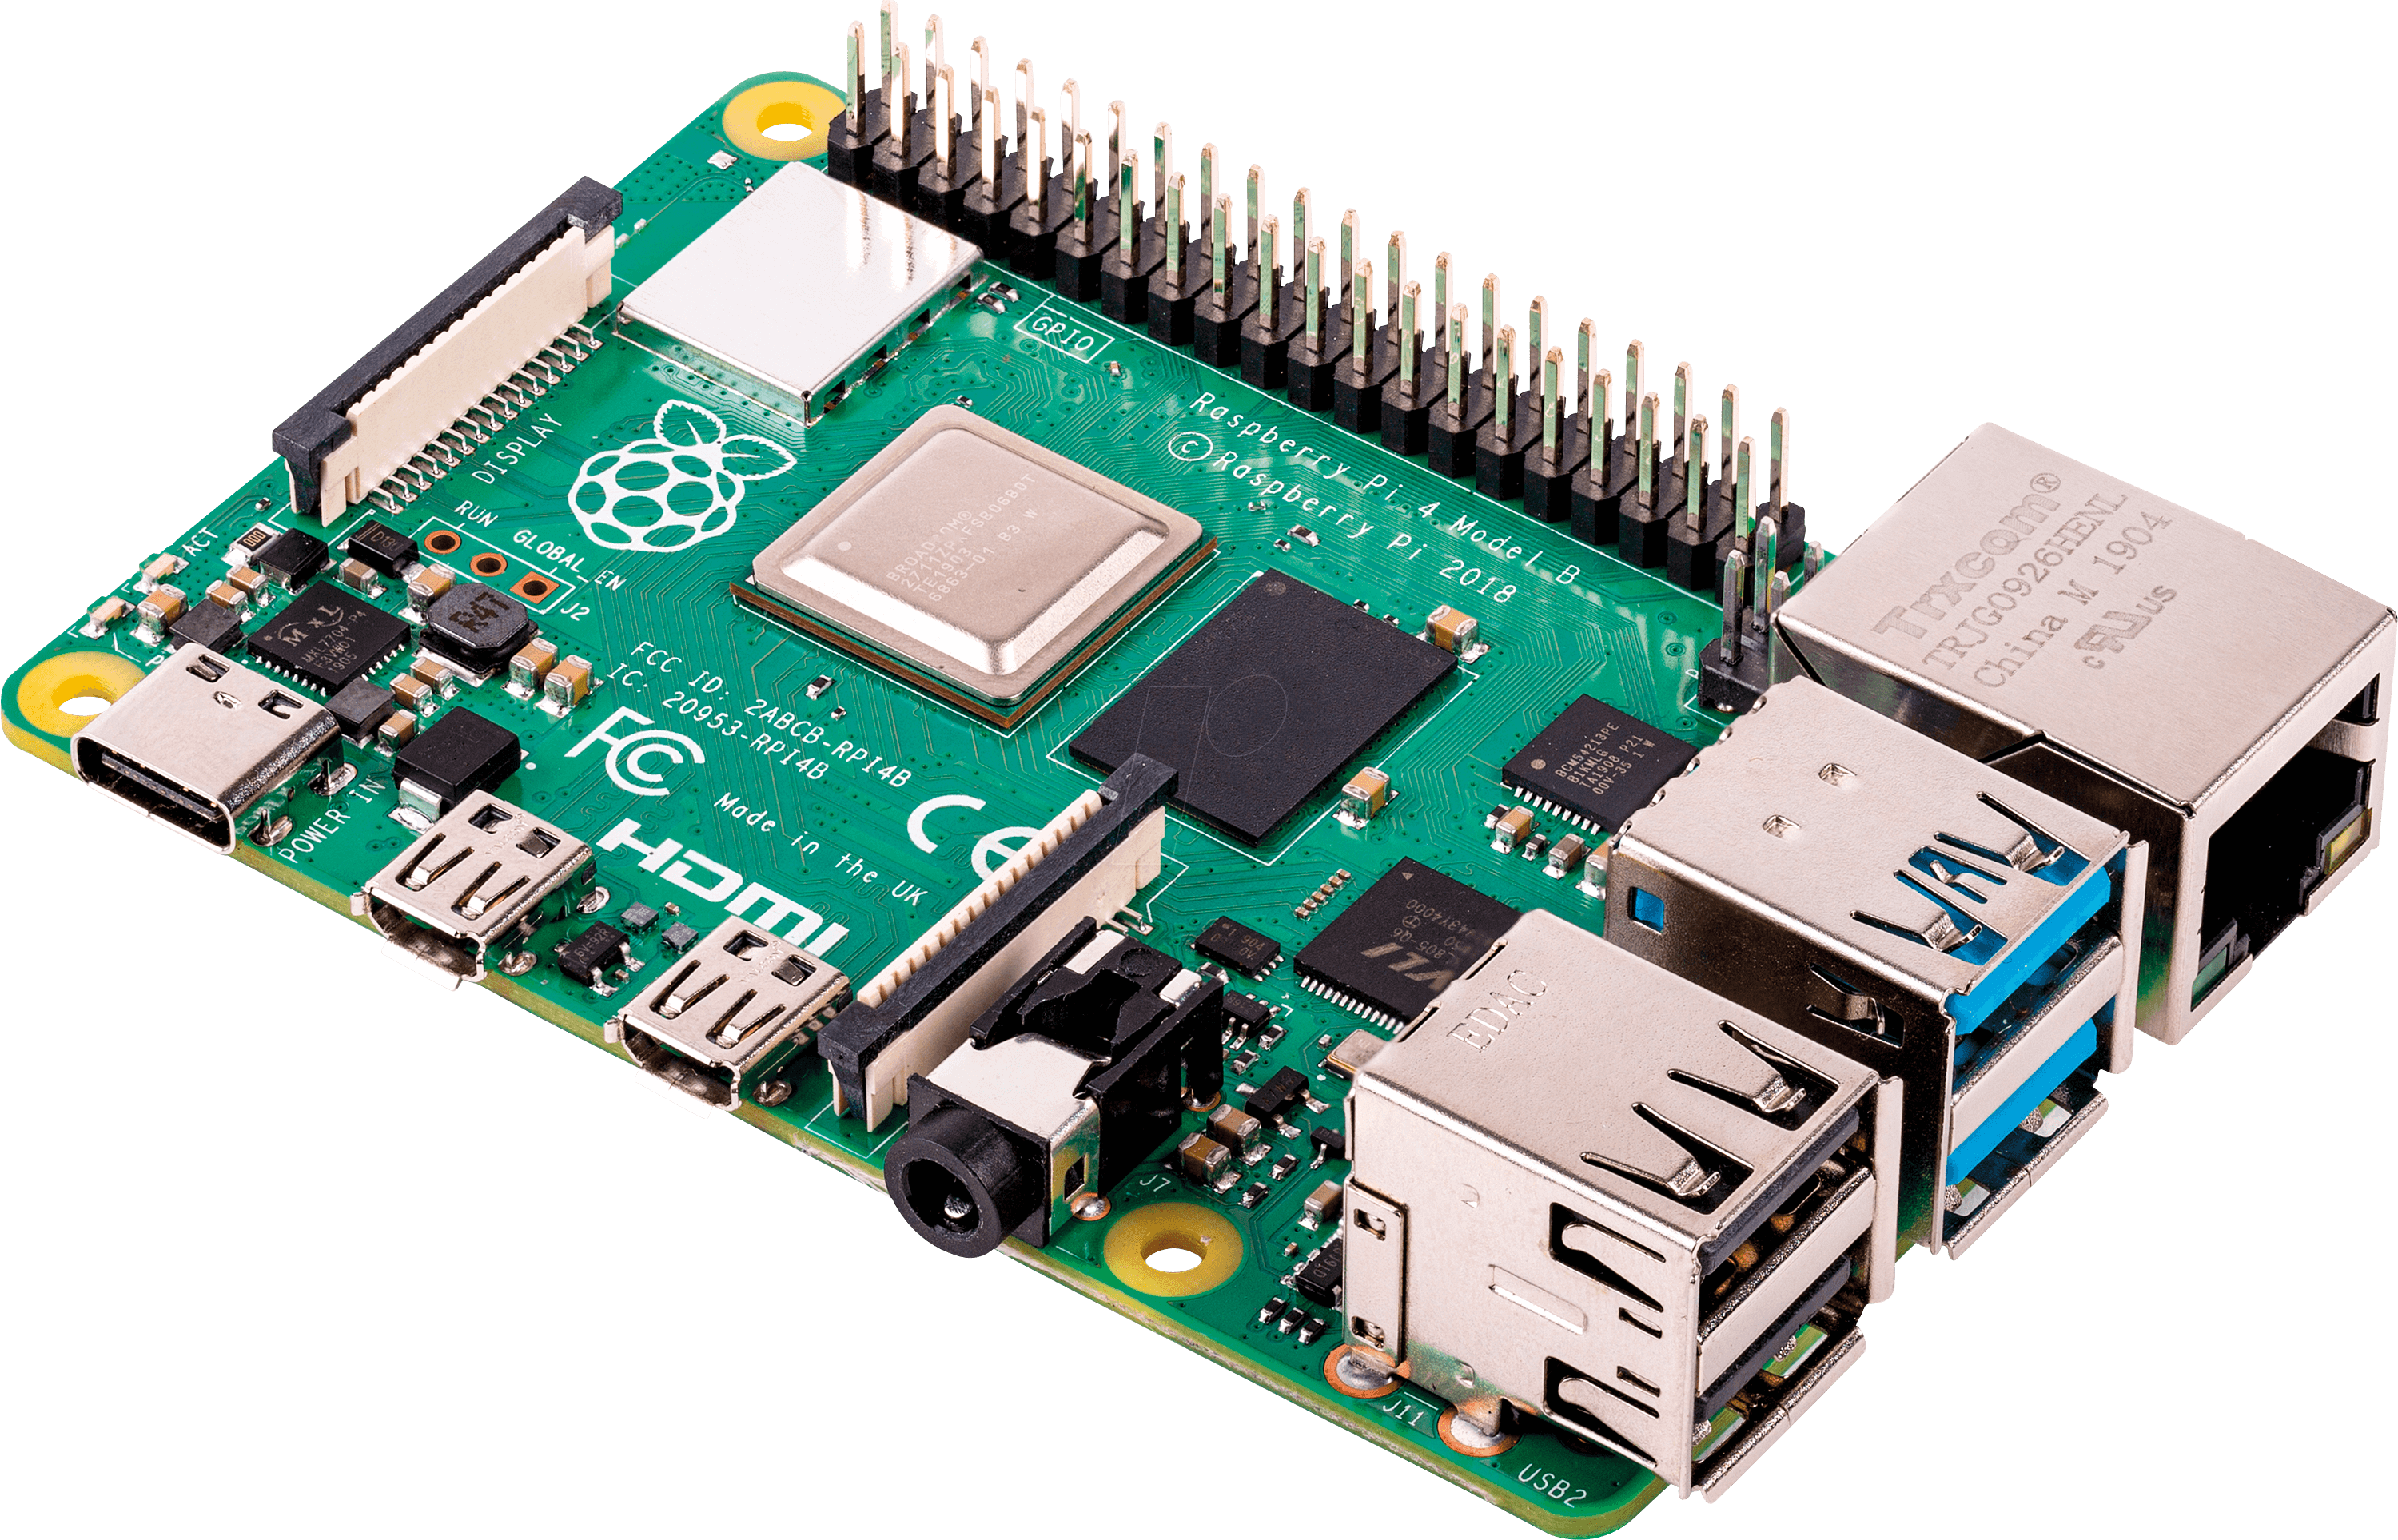
\includegraphics[width=0.6\textwidth]{Bilder/raspberrypi_4.png}

    \end{columns}
        
\end{frame}




\begin{frame}{NCS2 und Myriad Chip}

    \begin{columns}[T]
        \column{0.5\textwidth}
        \begin{block}{Funktionsweise}
            \begin{itemize}
                \item schnelle NN berechnungen
            \end{itemize}
        \end{block}
    
        \begin{block}{Anwendungen}
            \begin{itemize}
                \item für edge systeme
                \item vgl zu cloud basierten nns
            \end{itemize}
        \end{block}

        \column{0.5\textwidth}
        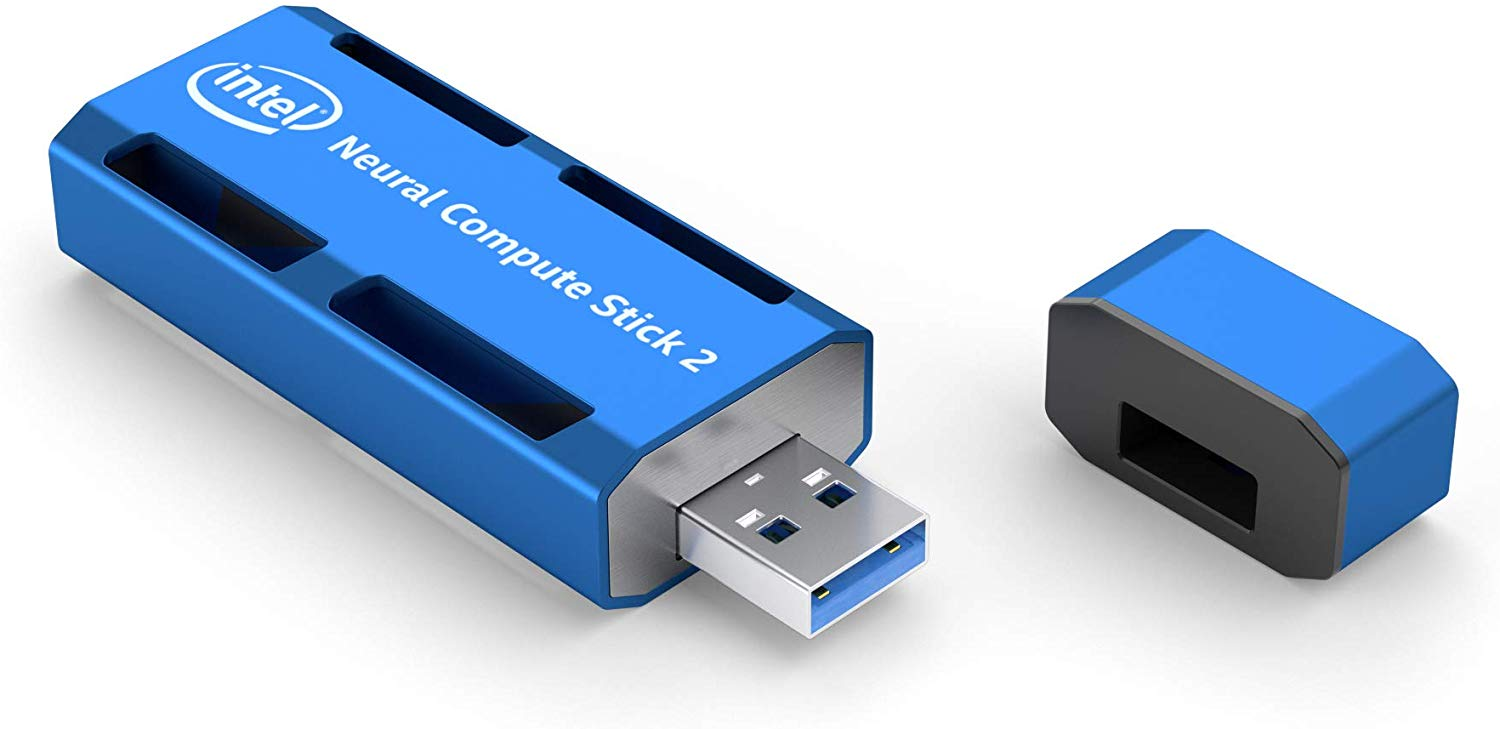
\includegraphics[width=\textwidth]{Bilder/ncs2.jpg}


        
    \end{columns}


    
\end{frame}


\begin{frame}{OpenVino}
    
    \begin{block}{\vspace{1cm}Open Vino Toolkit Developement Workflow}
        \begin{columns}[T]
            \column{0.3\textwidth}
            
            \begin{itemize}
                \item in Tensorflow, Caffe, rainierte Modelle
                \item Asymchrone Inferenz möglich
            \end{itemize}
            

            \column{0.7\textwidth}
            \begin{center}
                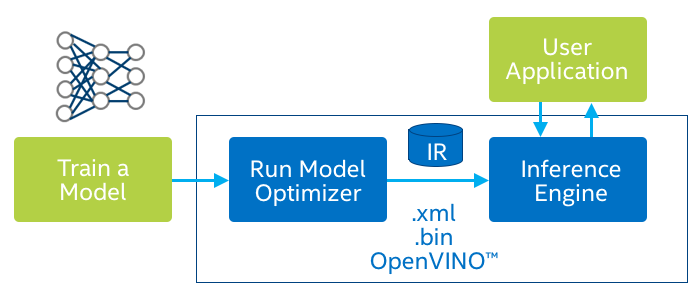
\includegraphics[width=0.9\textwidth]{Bilder/open_vino_workflow_steps.png}    
            
            \end{center}
        
        \end{columns}

        
    \end{block}

        
    
\end{frame}

